
\documentclass[letterpaper,twocolumn,10pt]{article}


\usepackage{times}            % standard fixed width font
\usepackage{usenix}

\usepackage{graphicx}
\usepackage{amsmath}
\usepackage{xspace}
\usepackage{footnote}
\usepackage{cite}
\usepackage{amsfonts}
\usepackage{subfig}
%\usepackage{natbib}
\usepackage{hhline}
%\usepackage{multirow}
\usepackage{setspace} 
\usepackage{epsfig}
\usepackage[hyphens]{url}
\usepackage[colorlinks,linkcolor=blue,citecolor=blue,urlcolor=blue]{hyperref}
\usepackage[hyphenbreaks]{breakurl}
\usepackage{booktabs}
%\usepackage[compact]{titlesec}
\usepackage{xcolor}
%\usepackage[algoruled,vlined,ruled,linesnumbered]{algorithm2e}
\usepackage{lipsum}
\usepackage{listings}

\usepackage[T1]{fontenc}
\usepackage[scaled=0.78]{DejaVuSansMono}
\lstset{
  language=C,
	basicstyle=\footnotesize\ttfamily,breaklines=true
}

\clubpenalty=10000      % penalty for creating a club line at end of line.
\widowpenalty=10000     % penalty for creating a widow line at top of page.

% Select one or other if want to see comments.
% \com is sometimes displayed during draft.
\long\def\com#1{}
%\long\def\com#1{{\bf \sc comment: }{\small [#1]}{\bf \sc\ endcomment}\newline}

\long\def\ennan#1{{\color{blue}{\bf Ennan: }{\small [#1]}}}
\long\def\ruzica#1{{\color{red}{\bf Ruzica: }{\small [#1]}}}
%\long\def\xxx#1{}

% Use this macro to force page breaks where ugly widows/orphans occur;
% be sure to recheck all uses after any significant change to the text!
\def\widowpage{\pagebreak}

% Choose abbreviated or long-version alternatives in paper
%\long\def\abbr#1#2{#1}			% abbreviated version
\long\def\abbr#1#2{#2}			% long version

% Choose abbreviations or long names/titles in bibliography
%\def\bibbrev#1#2{#1}			% short version
%\def\bibbrev#1#2{#2}			% long version
\def\bibbrev#1#2{\abbr{#1}{#2}}		% follow abbr macro

% Abbreviated or full citation lists: \abcite{basic}{others}
\newcommand{\abcite}[2]{\abbr{\cite{#1}}{\cite{#1,#2}}}

% Conference abbreviations: \bibconf[Nth]{SOSP}{Symposium on ...}
\newcommand{\bibconf}[3][]{#1 \bibbrev{#2}{#3 (#2)}}

\newcommand{\ie}{{\em i.e.\xspace}}
\newcommand{\eg}{{\em e.g.\xspace}}

% system related terms
\newcommand{\app}{ConfVer\xspace}

% Fault graph terms

\newcommand{\para}[1]{\smallskip\noindent {\bf #1}}

\begin{document}

\special{papersize=8.5in,11in}
\setlength{\pdfpageheight}{\paperheight}
\setlength{\pdfpagewidth}{\paperwidth}

% Uncomment one of the following two, if you are not going for the 
% traditional copyright transfer agreement.

%\exclusivelicense                % ACM gets exclusive license to publish, 
                                  % you retain copyright

%\permissiontopublish             % ACM gets nonexclusive license to publish
                                  % (paid open-access papers, 
                                  % short abstracts)

%\titlebanner{banner above paper title}        % These are ignored unless
%\preprintfooter{short description of paper}   % 'preprint' option specified.

\title{An Automatic Verification Framework for Software Configurations}

\author{~}

\maketitle
%\vspace{-50pt}


\section*{Abstract}

System failures resulting from configuration errors 
are major reasons for compromised availability and
reliability of today's software systems.
Although many misconfiguration handling techniques
such as checking, troubleshooting, and repair
have been proposed, 
offering automatic verification for configuration files -- as often  
done for regular programs -- is still an open problem.
This is because software configurations are typically written in
poorly structured and untyped ``languages'', and 
specifying constraints and rules for configuration 
verification is non-trivial in practice.

This paper presents \app, the first automatic verification framework for
general software configurations.
\app verifies a target configuration file $F$ through three steps.
Firstly, \app analyzes a dataset containing many sample configuration 
files belonging to the same system as $F$,
translating these sample files to a
well-structured and probabilistically-typed 
intermediate representation.
Secondly, \app derives rules and constraints by analyzing
this intermediate representation, thus building a
sophisticated language model.
Finally, \app uses the resulting language model to verify $F$.
The \app framework is highly modular, 
does not rely on system source code, and
can be applied to any new configuration file type with minimal user input. 

\app is capable of detecting various errors that cannot
be detected by previous efforts,
including entry ordering errors, fine-grained value correlation errors, 
and missing entry errors. 
We evaluate \app using a real-world dataset with 261 incorrect 
MySQL configuration files,
and \app is able to correctly 
detect errors (previous work failed to
detect) in 217 files.


\section{Introduction}
\label{sec-intro}

Configuration errors are one of the most important root causes of
today's software system failures~\cite{xu15systems, yin11anempirical}.
For example, Yin {\em et al.}~\cite{yin11anempirical} report
that about 31\% system failures were caused by misconfiguration problems and only 20\% were caused by bugs in program code. 
Misconfigurations, in practice, may result in various
system-wide problems, such as security vulnerabilities, 
application crashes, severe disruptions in software
functionality, and incorrect program executions%
~\cite{zhang14encore, yuan11context, xu13do, xu15hey}.  

While many efforts have been proposed 
to check, troubleshoot, diagnose, and repair configuration errors%
~\cite{attariyan10automating,
su07autobash, whitaker04configuration},
those tools mainly try to understand {\emph{what}} caused the error ---
they are still not on the level of
automatic verification tools used for regular program 
verification~\cite{Leino10Dafny, PiskacWZ14, BobotFMP15}.
Nevertheless, automated verification of configuration 
files would be highly
desirable~\cite{wang04automatic, zhang14encore, xu15systems}.
Two main obstacles why we cannot simply apply the existing automatic 
tools and techniques to verification of configuration files are: 1) a lack
of a specification which would describe properties of configuration files, and 2) a program structure of configuration files -- they
are mainly a sequence of entries assigning some value to system variables. The language in which configuration files are written does 
not adhere to a specific grammar or syntax. In particular,  the
entries in configuration files are untyped. Moreover, there are surprisingly few rules specifying constraints on entries and there
is no explicit structure policy for the entries.

In order to overcome all these obstacles,
researchers have proposed 
statistical analysis and learning based approaches%
~\cite{wang04automatic, zhang14encore, yuan11context}. 
These efforts build checking policies by learning a sample 
data set, rather than explicitly specifying entries' types or rules.
In particular, for each entry in a certain configuration file, 
if it deviates from the common values used in a large collection
of configurations (\ie, the data set for training), it is typically
suspected as a potential configuration error.
However, because these learning 
efforts {\em either} are limited to simplistic 
configuration errors (\eg, type errors and syntax errors), 
{\em or} heavily rely on template-based inference~\cite{zhang14encore}, 
many sophisticated configuration errors, 
\eg, hard to be templated in practice, cannot be detected.
For example, if {\tt extension = mysql.so} appears 
before {\tt extension = recode.so} in PHP configuration file,  
it would lead to a crash error, since the correct ordering 
should be {\tt extension = recode.so} before 
{\tt extension = mysql.so}~\cite{yin11anempirical};
however, such an error cannot be detected by existing
learning efforts, since it is hard to build a template for this
error~\cite{xu15systems}.

%Offering automatic verification to configuration files -- like
%what we did to programs -- has been advocated as a reasonable means
%to check the correctness of configuration files of interest.
%Nevertheless, it is still an open problem, because 
%1) software configurations are typically written in poorly structured 
%and untyped languages, and 2) writing specifications or constraints
%for configuration verification is non-trivial in practice.

In order to truly achieve automatic configuration verification,
we argue that we need to leverage a collection of more powerful learning 
algorithms (not necessarily depending on templates) to derive 
a more sophisticated language model (with abundant rules covering
tricky configuration errors), and then check the configuration files
of interest through the learned language model.

Based on the above argument, 
this paper presents \app, the first automatic verification framework
for general software configurations.
In particular, \app's workflow to verifying a given configuration file
could be looked as a three-step methodology.
First, \app analyzes a dataset containing sample configuration files,
thus generating a well-structured and probabilistically-typed 
intermediate representation.
Second, \app derives rules and constraints by analyzing
the intermediate representations, thus building a language model.
Finally, \app uses the resulting language model
to verify the given configuration file and detect potential errors.
Compared with previous efforts,
\app does not necessarily rely on users' templates, 
and is capable of detecting more tricky configuration errors that
cannot be identified by existing work (details in $\S$\ref{sec-motiv}). 

Building such an automatic verification framework for
configuration files, nevertheless, requires addressing several challenges. 
First, in order to formulate a correct language model, 
we need to infer each entry's type in a given configuration file;
however, the type of a variable cannot always be fully determined 
from a single value. 
For example, an entry {\tt foo = MAX\_SIZE} is most likely
an integer rather than string; however, existing type inference 
work would report this is an error, because foo should be assigned
an integer~\cite{zhang14encore}. We address this problem by introducing 
so called {\emph{probabilistic types}}.
Rather than assigning only one variable to a single type, 
we assign several types with their probability distributions. 
The entry in the above example might be assigned 
a probabilistic type like 
{\tt \{foo, MAX\_SIZE, [(Int, 60\%), (String, 40\%)]\}}.
With such probabilistic types in hand,
we can generate a more accurate language model,
thus significantly improving our checking capability.

Second, without template, how to learn rules and constraints present
a difficult. \ennan{Here, we need to add one-paragraph description 
to illustrate how we learn rules without templates, 
or why we say our learning results are better than existing
learning approach, \eg, EnCore.}

\com{First, given the fact that 
different systems' configuration files use various representations, 
the cost of introducing a completely new configuration
language (or representation) to instead of all these existing format looks 
like an impractical goal. This is not only because administrators need 
to learn this new language, but also changes existing system
infrastructure to support such a new language. 
In order to avoid the above issues, we propose a representation,
which is a type-based representation and 
much more structured than existing configuration format, 
but use it as an intermediate layer. We, at the same time,
develop many pluggable parsers
that can transform different systems' configuration representations
into our proposed intermediate representation for the post process.}

From a practical perspective, 
\app introduces no additional burden 
to the users: they can simply use \app to check for errors in their
configuration files. However, they can also easily extend the framework
themselves. The system is designed to be highly modular. If there is a
class of rules that \app is not currently learning, the user can develop
their own templates and learners for that class. The new learner can be
added to \app and this way it can check additionally a new set of
errors.

Our \app prototype still has a few limitations:
for example, we cannot handle configuration errors that can be only
triggered in system execution time.
Nevertheless, we believe \app may suggest a practical path
toward automatic and modular language-based configuration verification.
To summarize, this tool paper makes the following contributions:

\com{
Finally, from a systems perspective this is the first approach that {\emph{proactively}} checks 
 the correctness of configuration files. All previous work
~\cite{xu15systems,zhang14encore,yuan11context, wang04automatic,attariyan10automating,
su07autobash,whitaker04configuration} tries to identify the problem after the
failure occurred. Our approach isolates potential errors before the system failure occurs, e.g. before the installation. We can also see \app as a tool that can run in conjunction with existing tools. Pre-analyzed configuration files are already free from language-based errors, and this way the workloads of post-failure forensics at the runtime
is significantly reduced, thus making these tools truly practical.
}


\begin{enumerate}

\item We propose the first automatic configuration verification
framework, \app, that can learn a language model from an example set of 
correct configuration files, and then uses this language model to verify 
interested configuration files.
 
\item \app proposes probabilistic types to assign a confidence 
distribution over a set of types to each entry, 
while generating the intermediate representation. 

\item \app employs a collection of machine learning algorithms to 
enable powerful rule and constraint inference without the assistance 
from any pre-defined templates.

\item \app is capable of detecting various tricky errors that cannot
be detected by previous efforts,
including ordering errors, fine-grained value correlation errors, 
entry missing errors, and environment related errors. 

\item We implement a \app prototype and evaluate it by
conducting comprehensive experiments.

\end{enumerate}

\section{Motivating Examples}
\label{sec-motiv}

In this section we present the capability of \app through 
detecting errors in several real-world misconfiguration examples. 
These examples were non-trivial configuration errors
that were reported on StackOverflow~\cite{stackoverflow},
a popular question and answer website for programmers and administrators. 
%To better understand these problems, 
%we explored and analyzed misconfigurations 
%on a large number of user forums and on-line discussion sites.

\para{Example~1: Ordering error} 
Ordering errors were reported by Yin {\em et al.}~\cite{yin11anempirical} and our first
example illustrates how ordering errors can cause a system to crash. When a user configures PHP 
to run with the
Apache HTTP Server, most likely the user will take some already existing configuration files and adapt them
to suit her needs. The configuration file might contain, among others, 
the following lines:

\begin{lstlisting}[language=C, xleftmargin=.01\textwidth]
    extension = mysql.so
        ...
    extension = recode.so
\end{lstlisting}

This configuration file will cause the Apache server to 
fail to start due to a segmentation fault error. 
This is because, when using PHP in Apache, the extension {\tt mysql.so} 
depends on {\tt recode.so}, and their relative ordering
is crucial. 
We call the above example of a misconfiguration file
an {\em ordering error}.
Yin {\em et al.} report that ordering errors widely exist in
many system configurations, \eg, PHP and MySQL,
and typically lead to multiple system crash events.
However, no existing tool can effectively solve 
or detect this problem~\cite{zhang14encore, xu15systems, xu13do}.

By invoking \app, the user can detect such a configuration error.
In particular, \app reports that {\tt recode.so} 
should appear before {\tt mysql.so}, as shown
below:
 
\begin{lstlisting}[language=C, xleftmargin=.01\textwidth]
    ORDERING ERROR: Expected "extension=recode.so"
    BEFORE "extension=mysql.so"
\end{lstlisting} 

%TODO would be nice to have these as subsection or somehow be able to ref specific examples
\para{Example~2: Fine-grained integer correlation error}
\label{ex:fine}
Our second misconfiguration example~\cite{correlation} 
comes from a discussion on StackOverflow.
The user has configured her MySQL as in the following:

\begin{lstlisting}[language=C, xleftmargin=.01\textwidth]
    key_buffer_size = 384M
    max_heap_table_size = 128M
    max_connections = 64
    thread_cache_size = 8
        ...
    sort_buffer_size = 32M
    join_buffer_size = 32M
    read_buffer_size = 32M
    read_rnd_buffer_size = 8M
        ...
\end{lstlisting} 

The user complains that her MySQL load was very high, 
causing the website's
response speed to be very slow.
In this case, {\tt key\_buffer\_size} is used by all the threads
cooperatively, while {\tt join\_buffer} and {\tt sort\_buffer} are 
created by each thread for private use; thus, {\tt key\_buffer\_size},
\ie, the maximum amount of used key buffer, should be larger than 
{\tt join|sort\_buffer\_size} * {\tt max\_connections}. 
In the above example, however, it does not hold. 

If we run \app on this configuration file, \app  would return:

\begin{lstlisting}[language=C, xleftmargin=.01\textwidth]
  FINE GRAINED INTEGER RELATION ERROR:
  Expected "max_connections" * "sort_buffer_size"
               =< "key_buffer_size"
\end{lstlisting} 

The above example is a complex integer correlation, which implicitly
includes a computational correlation among different entries
in the configuration file.
We call these complex integer correlations as 
{\em fine-grained integer correlations}. 
Our tool can detect simple integer correlation---one entry's
value should have a certain correlation with another entry's 
value---as well.
For example, in MySQL, the value of {\tt max\_connections} 
should be higher than {\tt mysql.max\_persistent}.
While few existing tools~\cite{yin11anempirical, zhang14encore}
can detect the simple integer correlation errors,
to the best of our knowledge, \app is the first effort capable of
detecting fine-grained integer correlation problems.

\para{Example~3: Missing entry error} 
Many critical system outages result from the fact that an important
entry was missing from the configuration file. 
We call such a problem a {\em missing entry error}.
In a public misconfiguration dataset~\cite{configdataset},
many MySQL failure reports were caused by
missing entry errors.
Below is a real-world missing entry error example~\cite{yin11anempirical}:
when a user wants to use OpenLDAP to enable her directory access
protocol, she needs to use the password policy overlay. This is usually
achieved via the following entries in the OpenLDAP configuration file:

\begin{lstlisting}[language=C, xleftmargin=.01\textwidth]
    include schema/ppolicy.schema
    overlay ppolicy
\end{lstlisting} 

When using the password policy overlay in OpenLDAP, 
users must first include the related schema.
Leaving out the {\tt include schema/ppolicy.schema} entry, 
as done by many users~\cite{yin11anempirical}, 
causes the failure of LDAP. 
If the user runs \app on such a misconfiguration file,
\app would return:

\begin{lstlisting}[language=C, xleftmargin=.01\textwidth]
    MISSING ENTRY ERROR: Expected "overlay" "ppolicy"
    in the same file: "include" "schema/ppolicy.schema"
\end{lstlisting} 

\para{Example~4: Type errors} 
Many system availability problems are caused by 
assigning incorrect type of values to some key in configuration
files. Consider the following real-world misconfiguration
file~\cite{typeerror}: 
a user tries to install MySQL and she needs to initiate the path
of the log information generated by MySQL.
This user puts the following entry assignment in her MySQL
configuration file: 

\begin{lstlisting}[language=C, xleftmargin=.01\textwidth]
    slow-query-log = /var/log/mysql/slow.log
\end{lstlisting} 

Unbeknowest to this user, the entry ``slow-query-log'' should be an 
integer, not a string. This misconfiguration will lead to 
MySQL fails to start~\cite{querylog}. In MySQL, there is another entry 
named ``slow-query-log-file'' used to specify the log path.
With \app, this user can get the following result:

\begin{lstlisting}[language=C, xleftmargin=.01\textwidth]
    TYPE ERROR: Expected a Int with P=1.0 for
    "slow-query-log"
\end{lstlisting} 

%The above result means that we need to assign an integer value to
%the entry ``general\_log''. 

%
\section{Quantum Types}

Because our type inference is based on machine learning, we cannot be sure that a keyword unambigously has a single type.
This is an issue when we try to learn relational rules between keywords. 
Take the following file in the learning

foo = 300
bar = 300.txt


We want to learn the rule that $foo \in {substring(bar)}$, however using unambigous type inference, we would assign foo type int, and never try to generate a string relation rule for these two keywords.
By assigning foo a quantum type (e.g. ${Int <90\%>, String <10\%>}$), we can now generate rules for both types.

At runtime, when the user wants to check a file we update the probabilities one last time then 'collapse' the quantum type to a concrete type.
If the concrete type collapses to a Int, we consider the rules for ints, and vice versa.

This idea is closely related to exstentially quantified types.


\section{Learning strategy}

A primary concern in any machine learning type task is to minimize false negatives and false positives.
In the context of configuration file verification,
  a false positive is when \app reports an error on a valid confiuration file and
  a false negative is when \app fails to reports an error on an invalid confiuration file.
Too many false positives will cause users to ignore the reported error\cite{}.
However, since the cost of system failure is so high from a misconfiguration, \app propritzes the minimization of false negatives.

While a traditional classififcation learning machine learning approach can reduce both of these situations, there is can generally be no garuntee that all false negatives will be eliminated.
Instead of building classification models over the learning set (such as an SVM), we learn the largest set of rules that all correct configuration files satisfy.
In this way, \app can garuntee that, over the set of rules we consider, there will be no false negatives that could have been caught with the given learning set.
The only case of a false negative can be when there was no evidece of such a rule in the learning set - we cannot generate rules from nothing.
Framed as the question "Is this file valid", \app is complete but not sound. 

That is, taking the following definitions:
\begin{multline*}\\
\text{\{Considered Rules\}} = \forall files \in \text{\{Learning Set\}}, \{ r | r(files) = True \land r \text{ is non-trivial}\}\\
\text{\{Reported Rules\}} = {r | r(userfile)=False } \\
\text{\{True Rules\}} = \{r | \text{ if } r(userfile)=False \text{ then system crash } \land \\
   \exists file \in \text{\{Learning Set\}}, r(file) \text{ is non-trivial}\}
\end{multline*}

We have the following specification of \app.
\begin{multline*}\\
\text{\{True Rules\}} \subseteq \text{\{Considered Rules\}} \\
\forall r \in \text{\{True Rules\}}, if r(userfile)=False then \exists r \in \text{\{Reported Rules\}} \\
\neg \forall r \in \text{\{Reported Rules\}}, r \in \text{\{True Rules\}} \\
\end{multline*}

Another benefit to a rule based approach is that, unlike many classificaton models, \app can actually report the reason for failure, similar to a comiler for a programming language.
This is in contrast to neural nets for example, where we would just get a boolean value, and the mechanics of the system are entirly lost.
Reporting useful errors that specify a point of failure is important to help users fix their misconfigurations.

\section{Intermediate Representation}

Part of the reason configuration file errors are so common is because of the large number of different systems being used on the market.
Rather than proposing a new, unifying, configuration language (so that there would then be n+1 configuration languages), we use in intermediate representation language.
This allows us to reuse all our algorithms over any configuration file that can be convereted to the intermediate representation.
The portability of \app means that with very little intervtion, it can be widely used and adopted.

More grammatically complex languages tend to be harder to translation to an intermediate representation.
While there can be some context senestive structures in configuration files, we found it is easier to design the rule modules (Section \ref{}) to handle learning such structure, rather than encoding it in the intermediate representation.
Additionally, configuration files are generally grammatically simple, consisting mostly of a list of keyword-value pairs.
The keyword is the variable to be used in the system, and the value is the new value for that variable.

To specialize the converter for a particular language, a user must define a new language type, which simply acts as a flag for translation.
If a langauge requires specialized parsing, the user can write such code in the convert function based on pattern matching over the language type.
For example, the user must specify the delimiters of the language (characters for assignment and comments) for their new language. 

\section{Rules}

A core design principle in \app is modularity, so that a user can easily exentend it to their verification needs.
Rather than try to support every type of verification over configuration files, we provide a framework for defining new verfication properties.
We call each verification property a rule, for example the correct ordering of keywords or integer relationships between values.
These rules tend to be pairs of values with a relation.
For instance, an integer relation rule might be that the value of "foo" must be greater than the value of "bar".
It is also important that the rule has some empty value, to state that it is known there is no relation between the values.
This will prevent \app from trying to relearn rules when they have already been refuted.

These rules are represented as a type, where the type must support a particular interface (called a typeclass in Haskell) to be compatible with our system.
The typeclass can support anything that is Foldable, which roughly the user can use any datastructure.
In fact, in our implementation, two rules are implemented with lists, and two others use hashmaps.

\begin{lstlisting}
class Foldable t => Attribute t a where
  learn :: IRConfigFile -> t a
  merge :: t a -> t a -> t a
  check :: t a -> IRConfigFile -> Error
\end{lstlisting} 

The functions of this typeclass will be used, invisibly to the user, to make the overall system run.
As long as the specifications for each function are met, \app can garuntee completness.

\subsection{learn}
  For a single given file in the intermediate representation format, learn the full set of rules on that file.
  By overfitting to each file, we can eventually garuntee the completness of \app.
  The specification of this function is the obvious reduction of the Considered Set definition.

  $\text{learn } file =  \{ r | r(file) = True \land r \text{ is non-trivial}\}$

\subsection{merge}
  Merging the sets of rules from two files to build a new set that is true over both files is the most difficult and important function a rule must implement.
  This is generally implemented as a filter over the union of the two set, but may vary slightly.
  The formal specification of this method is that:
  \begin{multline*}
  \text{merge } Set1 \: Set2= \{r \mid \\
    r \in \text{Set1} \cup \text{Set2} \land \\
    \exists file \forall r' \in \text{Set1} \cup \text{Set2}, r(file) = True \land r'(file) = True \} \\
  \end{multline*}

\subsection{check}
  To check a file by using a rule set, we simply take all the rules that are releveant to the user's file.
  Rules that are relavent are the ones where both parts of the ordering are present.
  We learn the rule set for the user file, and every rule in the learned set must be present in the user file.

\section{Implementation}

\subsection{System}
Since we learn a set of rules on each file in isolation from the other, we have an embarrassing parallel situation.
Haskell allows us to easily take advantage of by using the parallel mapping library, parmap, both for translation to the intermediate representation, and for learning the rules on each file.
\xxx{merge can also be parallelized, but i haven't done it yet and might not get a chance}

\begin{lstlisting}
learnRules :: [ConfigFile Language] -> RuleSet
learnRules fs = let
  fs' = parMap rseq convert fs
  rs = parMap rdeepseq findAllRules fs'
 in
  foldl1 mergeRules rs
\end{lstlisting}

\subsection{Type Error Rules}
This builds a map between keywords and types, using the values as evidence.
see quantum.tex for more
i will write more on this tomorrow.

\subsection{Integer Relation Rules}
we only consider the relations , (==), (<=), (>=) because they are easy to pass aroud (as actual functions) in haskell.
We also committed cardinal since and create an instance for equality over these functions.
instance Eq (Int->Int->Bool) where

With more engineering effort, this could be extened with the use of a SMT solver to create more fine grained relational rules.
From our experience, more specific rule are not really needed for integer relations in configuration files.
However an SMT solver approach would be particularly useful for relations on strings, especially when considering substring relations between filepaths.

\subsection{Ordering and Missing Entry Rules}
These are the simpiliest of all rules, just making a lot of pairs and seeing which pairs continue to appear over the learning set.

There is actually a bit of a catch in ordering though - we are not complete over ordering rules.
This is because only our implementation does not satisfy the specification for the merge function listed above.
The problem arises from the fact the configuration files may have non-unique keywords.
Therefor, in the follwoing file we will derive the valid, but conflicting rules ([client],port) and (port,[client]).
\begin{verbatim}
[client]
port = 3306
[mysqld]
port = 3306
\end{verbatim}
Our implementation of merge removes and conflicting rules for the running set.
By introducing a renaming pass in the initial parsing we may be able to solve this, but have not found a satisfactory solution yet.


\section{The \app Framework Overview}

\begin{figure*}[tbp] \centering
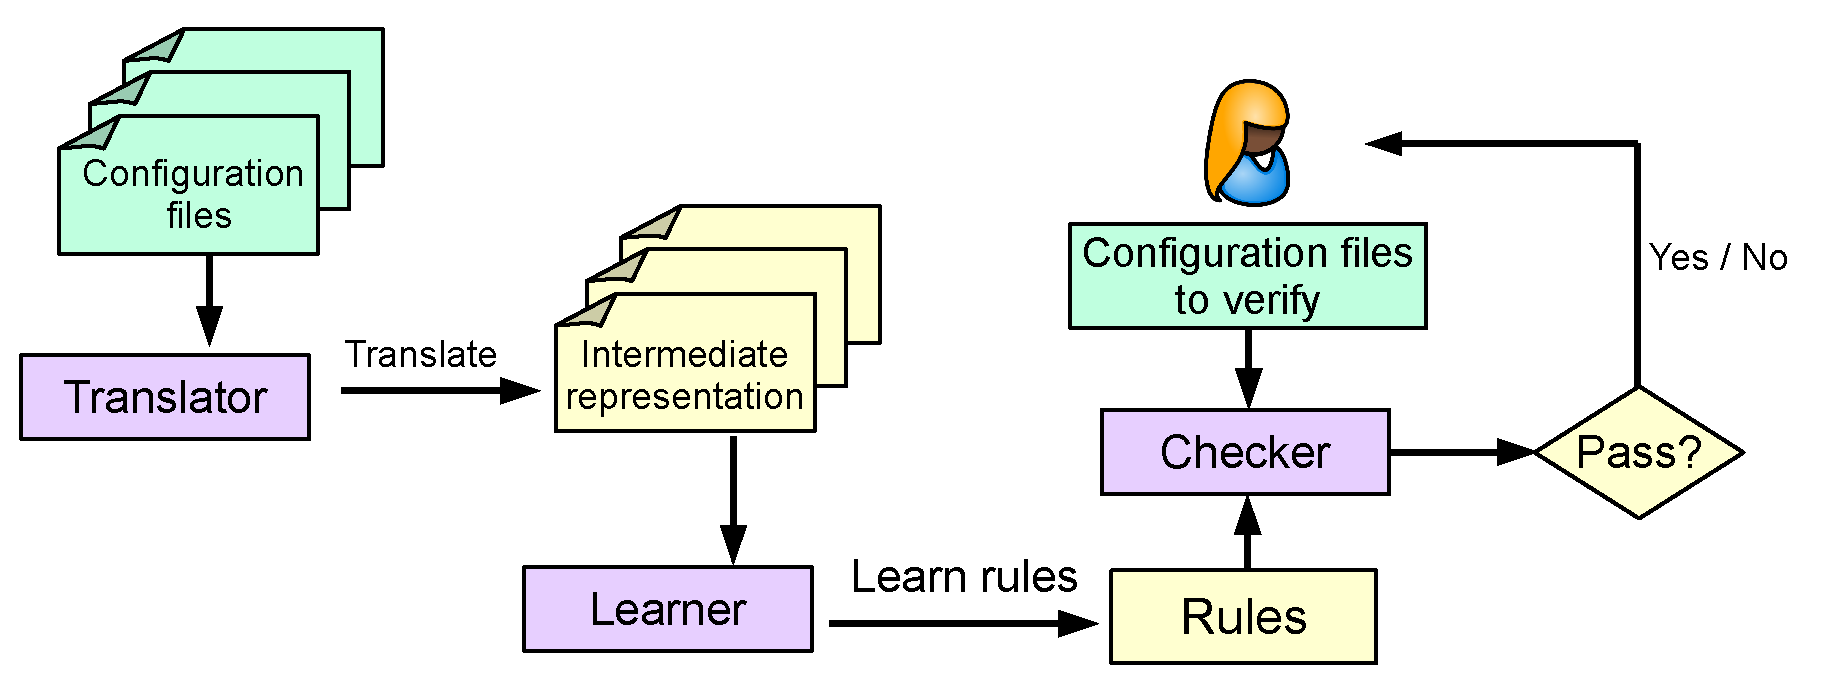
\includegraphics[width=0.88\textwidth]{figs/overview}
\caption{\app's workflow. The green components represent configuration 
  files, including both sample configuration datasets and users' input
  configuration files to verify. 
  The purple components are the modules of \app.
  Because template DB is not necessarily used, we use dashed
  arrow between it and the learner.
  Red boxes are sub-modules within the checker.
  The yellow components are results generated by \app's modules.}
\label{fig-overview}
\end{figure*}

We propose \app, an automatic verification framework,
which can solve configuration errors, \eg, ordering errors
and fine-grained value correlation, that previous work cannot tackle.
As depicted in Figure~\ref{fig-overview}, \app has three main steps:
translation, learning and checking. In this section, we briefly
describe how does each step work.

\para{Initial state.}
We start
with the assumption that we are given a number of (not necessarily) 
correct configuration files belonging to the same system, 
such as MySQL or Apache. 
Such files follow similar patterns, which we exploit
in a learning algorithm to build rules that
describe a language model for the files.

\para{Translator.}
The translator component first parses the input sample 
dataset (containing both configuration files and system environment
information), and then transforms them to a more structured
and typed intermediate representation.
When we run type inference on a configuration file, 
the type of a variable cannot always be fully determined from 
a single value.
We address this problem 
by introducing so called {\em probabilistic types}.
Rather than giving a variable a single type, 
we assign several types with their probability distributions. 
We can later use these more structured files
as a training set to learn the rules. 

\para{Learning.}
The learning algorithm is template-based to be easily extensible. 
We provide an initial set of templates and the
learner learns some concrete instances from the training set. These
rules are used for detecting errors violating the learned constraints
in the files given by the user.

As an illustration of a simple rule that we can learn, consider a template
 $X_1 \le X_2$, where $X_1$ and $X_2$ are
integer variables. The learner might derive the rule stating that
$\texttt{mysql.max\_persistent} \le \texttt{max\_connections}$. There is a classification and taxonomy of configuration errors in the 
existing work on automated configuration troubleshooting~\cite{yin11anempirical, configdataset}. We provide templates for every class that \app can handle: we consider integer constraints, ordering
constraints, typing constraints, and constraints about correlated entries (such as ``if $X$ is present, $Y$ has to appear as well''). 




\section{Translator}
\label{sec-trans}

The translator takes as input a sample dataset of configuration files and transforms it into another set of files written in
typed and well-structured representations.
The translator can be seen a parser, and it is only
used to generate an intermediate representation for post-processing, 
such as learning rules (see $\S$\ref{sec-learn}).
Coupled with rules generated by learner module,
we will have a complete language model to verify configuration files
of our interest.

Translating or parsing is system dependent. In other words, for MySQL
and HDFS, we need to develop different parsers to handle each of them,
respectively. \app allows users to 
provide extra help to the translator
for their specific system configurations,
but it is not required.

The majority of entries in a configuration files are assignments. Our first attempt was to simply
translate every key-value entry {\tt {k = v}} into a triple $(k, v, \tau)$, where $\tau$ is a type of 
$v$. However, sometimes we could not fully determine the type of key 
based on a single example value. For this reason, we introduced {\emph {probabilistic types}}.

Consider the following example.

\noindent{\tt {foo = 300}}\\
{\tt {bar = 300.txt}}

Most likely {\tt foo} should be an integer, but it could also be a string.
In the second case, we can learn the rule stating 
$ \texttt{foo} \in \textsf{substrings}(\texttt{bar})$. 
Instead of assigning one type to a value, the translator assigns a distribution of types 
to a value, an idea closely related to existentially quantified 
types~\cite{Launchbury93lazyfunctional}. 

Formally, we define probabilistic types as follows: let $\mathcal{T}$ be a set of basic types (cf. Table~\ref{table:kysymys}).
A probabilistic type built from $\mathcal{T}$ is a list of pairs 
$[(\tau_1, p_1),\ldots,(\tau_n, p_n)]$,
such that $\tau_i \in \mathcal{T}$, $0 \le p_i \le 1$ 
and $\Sigma p_i = 1$. 
These probabilities are updated each time a new example value 
for a key is encountered.

When a value has a probabilistic type, we generate rules for all its types.
This means that by assigning {\texttt{foo}} a probabilistic type 
(\eg, {\tt (\texttt{foo}, 300, [(\textsl{Int},90\%), 
(\textsl{String},10\%)])},
we would generate rules for both strings and integers.
Once the type inference can uniquely determine the type, 
the probability of all other types is set to zero, 
and the associated rules are withdrawn.

In \app, the set $\mathcal{T}$ contains strings, integers, file paths, 
sizes, and IP addresses. With every type, we associate a list of templates 
that are used to learn the rules about those files. Table~\ref{table:kysymys} contains
the most important types and templates.

\begin{table}
\caption{Table of types, along with associated templates, used in \app}
  \begin{tabular}{| l |  l |}
    \hline
    Type &  Template \\ \hline
    Integer & $X = Y, X\neq Y, X \leq Y, X < Y, X * Y < Z, \ldots $\\ \hline
    String & $\textsf{substr}(U, V), \textsf{prefix}(U,V), \textsf{suffix}(U,V), \ldots$   \\ \hline
    File Path & $\textsf{isFile}(F), \textsf{isDir}(D),\ldots$   \\ \hline
    Size & Similar to integers   \\ \hline
    Port & $P_1 > P_2$ \\ \hline
    IP Addr.  & $\textsf{sameSubnet}(addr1, addr2)$   \\
    
    \hline
  \end{tabular}
\label{table:kysymys}
\end{table}


In general, the templates works as follows: if there are two entries ${\tt {k1 = v1}}$ and 
${\tt {k2 = v2}}$, let $t(X, Y)$ be a template that can be applied to those values (w.r.t. their types).
If $t(v1, v2)$ holds, \ie, the template condition is valid for those concrete values, then we will add a rule
$t(k1, k2)$ to a list of potentially correct specifications. Note that the rule expresses a relation between variables.

With the help of probabilistic types, we addressed ambiguities during the parsing phase. Another problem that we need to solve
is that configuration files sometimes contain a simple version of the {\tt {if-then}}, such as in Apache HTTPD, that 
sets conditions for which an action should be applied. Therefore, we also add this guard to our entry 
during the parsing phase. We first check if the guard is true before deriving a rule; otherwise, we skip the entry.

To summarize, the translator translates every entity ${\tt {k = v}}$ in a configuration file into a quadruple entry
$$(g,k,v,\textsf{List}[p_1:\tau_1, \ldots, p_n:\tau_n])$$

For an entry, we denote the corresponding guard by $g(e)$, the key by $k(e)$, the value by $v(e)$, and the probabilistic
type list by $typelist(e)$. 

\com{Note that typing is also a system module than 
can be easily extended to support more types. 
In that case the user will need to provide rules for type inference 
and probability distributions for values where type inference is ambiguous.
}


\section{Learner}
\label{sec-learn}

The goal of the learner module is to derive rules and constraints from
the intermediate representation generated by the translator.
It has two components.
The first component ($\S$\ref{subsec-rules}) 
learns rules for checking misconfiguration errors like
missing entry, ordering, and fine-grained value correlation errors. 
These errors tend to cause total system failures.
%Once the configuration file has been validated against such rules, 
%the user may choose to invoke a more sensitive constraint checker. 
The second component ($\S$\ref{subsec-constraints}) 
aims to derive 
constraints on entries to check for suspicious (or anomalous) values 
that may violate standard practice. These anomalies can cause partial 
degradation of the system, such as significant reduction in performance, or even 
total failure as in Example~4 of $\S$\ref{sec-motiv}.

\subsection{Derivation of Probabilistic Rules}
\label{subsec-rules}

The first component learns rules that must hold over 
multiple parts of a configuration file.

\para{A strawman solution.}
We now first present a strawman solution (employed by
previous work~\cite{santolucitoCAV, zhang14encore}) that uses 
a set of correct configuration files as a learning set, 
from which it is possible to derive rules 
that must hold with absolute certainty. 
In practice, however, it is difficult to obtain a set of files 
that is both guaranteed to be without misconfiguration 
and large enough to learn many rules of configuration files.
This usually requires manual verification of the learning set, 
which is prone to error.

As a result of this restriction, 
these efforts only consider a rule if it holds over exactly every file in 
the learning set. This behavior can be formally described as follows:

\begin{small}
\begin{flalign*}
C =&\ \text{Correct Learning Set}\\
\text{::}\ & \text{\{Configuration Files in Intermediate Representation\}}\\
LR =&\ \text{Learned Rules :: \{Rule\}}\\
RR =&\ \text{Reported Rules :: \{Rule\}}\\ 
LR =&\ \{ r\ \mid \forall file \in C,\ holds(r,file)\} \\
RR =&\ \{ r\ \mid r \in L\ \land \neg\ holds(r,userfile) \}
\end{flalign*}
\end{small}

Each rule can be thought of as a mapping from 
lines $j$ and $k$ in a configuration file to a relation, $R$.

\[
\{ Rule = (a_j, a_k) | j \neq k \} \rightarrow \{ R \}
\]

Specifically, $a_j$ and $a_k$ are two different lines from our
intermediate representation, or more formally, $j \neq k \land
a_j, a_k \in \{ L \}$ where is the set of lines (key-value pairs) found
in the learning set. The relation $R$
is a Boolean function specific to the error to detect. 
As an example, to detect the error that key $k_1$ must always 
have a value greater than key $k_2$, the relation $R$ is $>$.

\para{Our approach.}
In \app's leaner module, the rule learning mechanism is tolerant 
enough to accept a dataset {\em full of} incorrect configuration files.
Rather than manually correcting each file, 
we extend the previous formalism to run probabilistic learning
on our intermediate representations (generated by the translator). 

Our probabilistic approaches for learning the entry missing, 
ordering, and fine-grained value correlation rules stem 
from existing work with building 
the non-probabilistic versions of these rule-learning algorithms. 
We start with the idea that for each of these rules, 
we are going to consider all possible pairs of keys that appear in every 
file, and for our learning process, calculate the likelihood that each of 
these pairs constitute a rule. 
In essence, this is a mechanism that will consider many different possible 
pairs of lines of entries in the file, 
and attempt to compile a set of these pairs 
that are expressed more often than others as a basis for finding patterns 
within the example set that can be used to evaluate new files.

More formally, this approach can be defined as follows. 
The output of our learning algorithm is augmented to a map from 
key-value pairs to a probability distribution over number of possible 
relations.

\[
\{ P\_Rule = (a_j, a_k) | j \neq k \} \rightarrow \{ (R_1, R_2, ... , R_n) \}
\]

We can think of each of these $(a_j, a_k)$ as possibly having a different relationship, defined by the set $\{ R_i \}$, which cover the entire outcome space of possible relationships between the two values $(a_j, a_k)$.

For the entry missing rules, we define $R_1$ as the event that $a_j$ and
$a_k$ appear together, and $R_2$ to be the event that $a_j$ appears
without $a_k$, or by the transitive equivalent, $a_k$ appears without
$a_j$. For the ordering rules, we define $R_1$ as the event that
$a_j$ appears before $a_k$ and $R_2$ be the event that $a_k$ appears
before $a_j$. For the value correlation rules, we define $R_1$ as the
event that $a_j \leq a_k$, $R_2$ the event that $a_j = a_k$, and $R_3$
the case that $a_j \geq a_k$. Notice that the $R_i$ do not have to be
disjoint, but only have to union to the entire probability space.

By examining the learning set, we will derive a distribution of the set $\{R_i\}$ based on how many times we observe an occurrence of each relation. This distribution will then be used at checking time to determine if a user's configuration has broken a likely rule. 

\begin{small}
\begin{flalign*}
I\ \ =&\ \text{Incorrect Learning Set}\\
\text{::}\ & \text{\{Configuration Files in Intermediate Representation\}}\\
LP =&\ \text{Learned Probabilistic Rules :: \{(P\_Rule)\}}\\
RP =&\ \text{Reported Probabilistic Rules :: \{(P\_Rule)\}}\\
LP =&\ \text{count\_relation\_occurrences}(I)\\
RP =&\ \{ r\ \mid r \in LP\ \land \Pi(r)>p \land \neg r(userfile) \}
\end{flalign*}
\end{small}

A rule will be reported as broken if the probability the rule is correct, $\Pi$, is greater than some user defined constant, $p$. This constant can be adjust to the user's preference. A small $p$ will increase the likelihood of finding an error, but also increase the number of false positives that are reported.


\subsection{Learning Suspicious Constraints}
\label{subsec-constraints}

With a configuration file that has been verified against catastrophic
failures (\eg, entry missing, type and ordering errors), 
the user may also want to find out more subtle issues.
Anomalous values can cause tricky, but impactful, performance and memory
issues that are hard to debug, as discussed in Example 4 of 
$\S$\ref{sec-motiv}. 
Consequently, anomalous values should be flagged and a warning returned
to the user indicating the violation.

We now describe the technique we use to detect anomalous values for 
numerical attributes. Let $A$ be the set of attributes contained in the 
configuration files in the sample dataset. 
Let $A_n$ be the subset of attributes of $A$ which are numerically typed. 
Then, for each attribute $a \in A_n$, we construct a vector $v_a$ of the 
values corresponding to attribute $a$, seen over the entire sample dataset.
For each $v_a$, we compute 
an interval  $$[\hat{v_a} - 50*MAD(v_a), \hat{v_a} + 50*MAD(v_a)],$$ 
where $\hat{v_a}$ represents the median over the values 
in $v_a$ and $MAD(v_a$) refers to the 
median absolute deviation. 
This is a variant of a standard outlier detection test, namely the Hampel identifier.\footnote{Mathematically, $MAD(v_a) = 1.4826* median(|v_a - \hat{v_a}|)$, estimating standard deviation 
for a normal distribution.} 
In the checking phase, as long as the checker finds a value for a numerical 
attribute in the checked file outside of this interval, 
a warning would be printed to the user indicating the violating value, 
the attribute, and the upper or lower Hampel threshold. 

The intuition behind this is that if the user has input a value 
that falls outside of an interval containing values that are considered 
``normal'' over the entire sample dataset, 
that value will probably cause an error, in particular for performance. 
We cannot know for sure if this value will cause an issue. 
For instance, a user might have a machine with 
particularly high-end hardware, 
in which case a value beyond the upper Hampel threshold may be appropriate. 


\section{Checker}
\label{sec-checker}

With the learned rules and constraints in hand (generated
by the learner module),
\app checks whether any entry in a target configuration file
violates the learned rules and constraints.
For a given configuration file, \app parses it using the same
way employed in the translator, thus obtaining a structured
and typed representation for the target configuration file.
Then, the checker uses the two sub-modules (shown in 
Figure~\ref{fig-overview}) to check the target
configuration file based on rules and constraints.

\para{Error detecting.}
The first sub-module of our checker,
named error detecting in Figure~\ref{fig-overview}, 
is able to detect the following errors:
entry missing errors, ordering errors, 
correlation errors (including fine-grained value correlation errors),
type errors and system environment errors (depending on templates).
In particular, the checker just see whether the representations 
parsed from the target configuration files violate our
learned rules.

\para{Anomaly checking.}
This checking occurs in the second sub-module of the checker.
Different from the previous checking tasks,
suspicious warning is just to detect whether some value
is too different (or distinguished) from the same entries in the
training dataset. Even if some values are statistically different
from the ones in the training dataset, 
it does not mean such a value is incorrect;
thus \app, in this case, throw out a warning to the user who
enters the target configuration file, and a report containing 
normal values in the training dataset.
\app allows users to choose whether they want to change 
the values according to the ones in the training configuration
files or not.


\section{Discussion and Limitations}

This section discusses a few \app's limitations
and possible solutions.

\para{Legal misconfigurations.}
While \app can check for diverse configuration errors without
human intervention, most of the existing proactive 
misconfiguration detection techniques,
including \app, cannot handle configuration errors
resulting from events occurred during the system runtime.
Such configuration errors are referred to as {\em legal misconfigurations}%
~\cite{yin11anempirical}. In particular, 
many parameter misconfigurations have 
perfectly legal types and values, 
but do not deliver the functionality intended by users. 
For example, after a website's traffic significantly increases,
the parameter {\tt Max\_key\_buffer} in MySQL may not 
be able to handle increasingly more data traffic,
thus leading to the outage of the whole system.
These cases are more difficult to detect by
automatic checkers and may require more user training or
better configuration design.
A potential solution is to combine existing misconfiguration diagnosis
tools, \eg, X-ray~\cite{attariyan12x-ray} 
and ConfAid~\cite{attariyan10automating},
with \app in order to enhance the 
misconfiguration checking capability.

\para{Misconfiguration across software components.}
As exposed by Yin {\em et al.}~\cite{yin11anempirical},
cross-software configuration correlation problems also account
for a considerable number of misconfiguration cases.
For example, in a LAMP-based Web server, one entry in 
PHP configuration file, {\tt mysql.max\_persistent = 400}
may make users encounter a ``too many connections'' error,
because a correlated entry in the underlying MySQL's configuration
file assigns {\tt max\_connection} to 300, which is less
than the MySQL connection numbers in PHP's configuration file (\ie, 400).
It is quite difficult to detect such a type of tricky error
through leaning approaches, because not only users or engineers 
are not aware of the hidden interactions~\cite{xu15systems},
but also it is hard to obtain a global knowledge to the entire
configurations due to the business privacy concerns of
each software provider.
One possible solution to this problem might be to introduce
some cryptographic protocol, \eg, private set
intersection~\cite{kissner05privacy}, to privately extract the
overlapping entries, \eg, {\tt mysql.max\_connection} in the 
above MySQL and PHP case, for double-checking.

\para{Network configuration verification.}
\app mainly focuses on software configurations, \eg, MySQL and Apache,
so that our approach is limited to support network configuration
verification. This is because network configurations have quite
different representations, format and rules from software configurations,
since network configurations are typically written in 
more domain-specific policy languages.
In fact, many network verification tools, 
\eg, NoD~\cite{lopes15checking} and 
Dobrescu {\em et al.}~\cite{dobrescu14software},
have been proposed to check whether network configurations
meet their specifications.

\para{More complex configuration structure.}
The current \app mainly targets key-value configuration files,
but in practice many systems, \eg, OpenStack~\cite{OpenStack},
employ very complex configuration format and structure,
which \app cannot handle.
Verifying such structurally complex configurations typically needs
\app to learn a much more sophisticated language model,
which is challenging in practice.
Recent efforts~\cite{raychev15predicting, raychev16learning} 
may present a possible solution on this limitation.
These techniques can learn a call-graph from a training program set,
and check a new program based on properties extracted from this
generated call-graph. If we look a structurally complex configuration 
file as a program in these tools, we may be able to use a similar way
to verify whether the configuration file violates any 
property of our interest. 


\section{Implementation and Evaluation}
\label{sec:eval}

We have implemented a tool, \app, and evaluated it based on real-world configuration files taken from Github.
\app is written in Haskell and is available open source at \textit{url redacted for anonymity}.
Thanks to the Haskell's powerful type system, the implementation can easily be extended with new rule classes or applied to different configuration languages with minimal change to the rest of the code base.
A user only needs to provide the functions for the rule interface (a typeclass in Haskell) to 1) learn relations from a single file 2) merge two sets of rules and 3) check a file given some set of rules.

\subsection{Evaluation}

To evaluate our \app prototype, we require a separate training set and test set. 
For our training set, \trainingSet, we use a preexisting set of 256 
industrial MySQL configuration files collected in previous configuration 
analysis work~\cite{configdataset}.
This is an unlabeled training set, though most of the files have some errors.
For our test set, we collected 1000 MySQL configuration files 
from Github, and filtered the incorrectly formatted files out for a final 
total of 973 files.
In our evaluation, we focus on MySQL for comparability of results, but \app can handle any configuration language (that can be parsed to the intermediate representation from Sec.~\ref{sec:trans}).

We report the number of rules learned from the training set and the number of errors detected in the test set in Table~\ref{table:learning}.
One interesting note is that without probabilistic types we learned 327 fine grained rules and detected 1367 errors.
By introducing probabilistic types, we remove 114 incorrect rules and thereby remove 1023 false positives.
We are guaranteed these are all false positives since there cannot be a correct rule of relating the types $size*size$ and $size$ because of the semantic interpretation of the $size$ units.

We also provide the support and confidence thresholds, $t_s, t_c$, used in this evaluation.
These number can be adjusted by the user as a slider to control the level of assurance that their file is correct.
Since these settings depend on both the user preference and training set quality, we simply choose values for which \app reports reasonably sized output.
This is a determined by the user by examining the rule set output over the training set.
Following common practice from association rule learning, initial values for support are confidence are generally 10\% and 90\% respectively.

We record the histogram of errors across the test set in Figure~\ref{fig:histo}.
This is intuitively an expected result from randomly sampling Github - most repositories will have few errors, with an increasingly small number of repositories having many errors.

\begin{figure}[h]
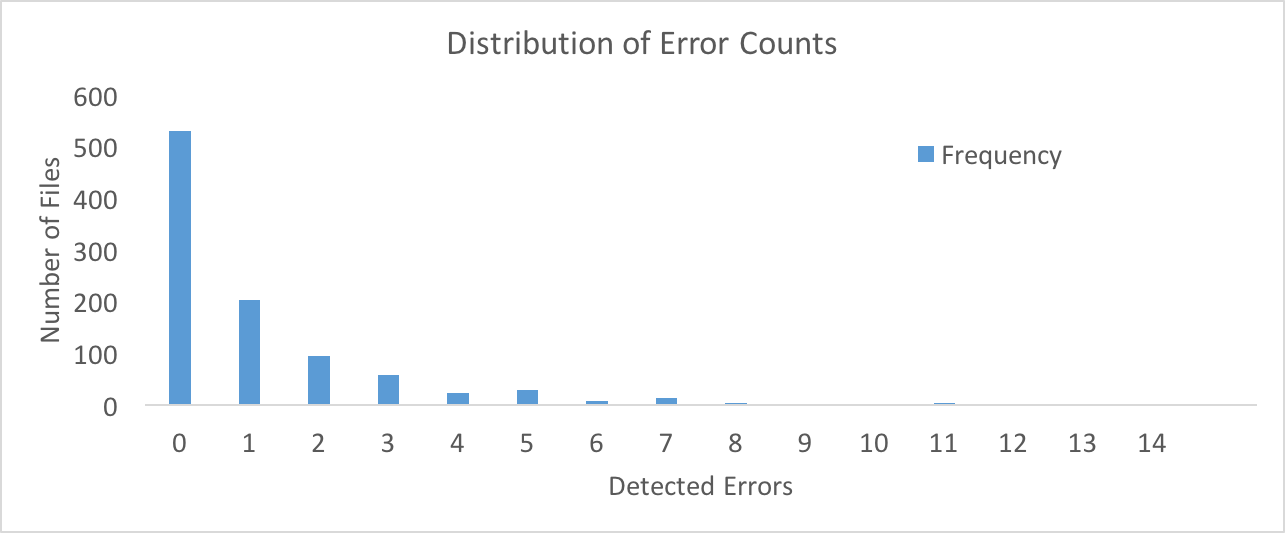
\includegraphics[width=\textwidth]{figs/histogram.png}
\caption{Histogram of errors - 14 errors were detected in 1 file}
\label{fig:histo}
\end{figure}

\begin{table}[h]
\centering
\caption{Results of \app}
\label{table:learning}
\setlength{\tabcolsep}{0.5em}
\begin{tabular}{|c|c|c|c|c|}
\hline
{\bf Class of Error } & {\bf \# Rules Learned} & {\bf \# Errors Detected} & {\bf Support} & {\bf Confidence}\\ 
\hline
\hline
Order        & 13  & 62   & 6 \%  & 94 \% \\ 
Missing      & 53  & 55   & 2 \%  & 71\% \\ 
Type         & 92  & 389  & 12 \% & 70\%  \\ 
Fine-Grain   & 213 & 324  & 24 \% & 91\%  \\ 
Coarse-Grain & 97  & 237  & 10 \% & 96\% \\ 
\hline 
\end{tabular}
\end{table}

The errors reported may have varying impacts on the system, ranging from failing to start, runtime crash, or performance degradation.
However, since \app is a probabilistic system, it is also possible that some errors are false positives, a violation of the rule has no effect on the system.
Note that in contrast to program verification, we do not have an oracle for determining if a reported error is a true error or a false positive.
While we can run a program to determine the effect a specification has on the success of compiling/running the program, no such test exists for configuration files.
Because configurations are dependent on the rest of the system (\ie, the available hardware, the network speed, and the usage patterns), we cannot simulate the all conditions to determine if a reported error will cause system failure.
As evidenced by Example~\ref{ex:fine}, some misconfigurations will only cause greater than expected performance degradation, and only under particular traffic loads.
In light of this, the definition of a true error is necessarily imprecise.

Although we cannot identify false positives, we can identify true positives by examining online forums, like StackOverflow.
On these forums we find reports that particular configuration settings have caused problems on real-world systems.
Furthermore, any error for which we can find evidence online is likely to be more problematic than errors that do not have an online record, 
  using the reasoning that this error has caused enough problems for people to seek help online.
In this case, we would like \app to sort the errors by their importance or potential severity.
To achieve this sorting we use the rule graph analysis metric described in Sec.~\ref{sec:ruleorder}.

To estimate the impact of this metric, we track the rank of known true positives with, and without, the augmented rule ordering in Table~\ref{table-casestudy}.
For this table, we picked the known true positive rules, listed in the Errors column, and pick configuration files in the test set that have these errors.
We picked 3 files for each true positive by choosing the files with the highest number of total reported errors in order to clearly observe the effects of our optimizations.
Although this gives a more clear picture of the effect of our optimizations, it results in a slightly inflated false positive rate.

We test the following conditions; just rule graph analysis (RG) to sort the errors, just probabilistic types to filter the rules (PT), and both optimizations at the same time (RG $\land$ PT).
For each entry we list X/Y, where X is the rank of the known true positive, and Y is the total number of errors found in that file.


\newcommand{\tablewidth}{6cm}
\definecolor{Gray}{gray}{0.80}
\newcolumntype{g}{>{\columncolor{Gray}}c}


\begin{table*}[tbp]
\centering
\caption{Sampled misconfiguration files for error detection evaluation.}
\label{table-casestudy}
\setlength{\tabcolsep}{0.5em}
\begin{footnotesize}
\begin{tabular}{|c|c|c|g|g|c|}
\hline
{\bf Errors} & {\bf URLs} & {\bf None} & {\bf PA} & {\bf PT} & {\bf PT$\land$ PA}\\ 
\hline
\hline
\multirow{3}{*}{\parbox{\tablewidth} {\scriptsize ORDERING ERROR: Expected ``innodb\_data\_home\_dir'' BEFORE ``innodb\_data\_file\_path''} }
& url & 12/12 & 3/12 & 5/5 & 3/5 \\
& url & 11/11 & 2/11 & 3/3 & 3/3 \\ 
& url & 9/9   & 3/9  & 4/4 & 3/4 \\ 
\hline

\multirow{3}{*}{\parbox{\tablewidth} {\scriptsize MISSING ERROR: Expected ``key\_buffer'' WITH [isamchk]} }
& url & 6/10 & 2/10 & 2/4 & 2/4 \\ 
& url & 2/3 & 3/3 & 2/3 & 3/3 \\
& url & 2/3 & 3/3 & 2/2 & 3/3 \\  
\hline

\multirow{3}{*}{\parbox{\tablewidth} {\scriptsize TYPE ERROR: Expected an integer for “slow\_query\_log”}}
& url & 32/34 & 1/34 & 5/7   & 1/7 \\ 
& url & 9/20  & 2/20 & 10/11 & 2/11 \\  
& url & 9/19  & 2/19 & 10/11 & 2/11 \\
\hline

\multirow{3}{*}{\parbox{\tablewidth} {\scriptsize FINE GRAINED ERROR: Expected \\ ``max\_connections'' * ``sort\_buffer\_size'' $\geq$ ``key\_buffer\_size''}}
& url & 30/34 & 18/24 & 6/7 & 3/7 \\ 
& url & 23/25 & 9/25  & 8/9 & 3/9 \\  
& url & 20/23 & 14/23 & 6/7 & 5/7 \\
\hline

\multirow{3}{*}{\parbox{\tablewidth} {\scriptsize INTEGER CORRELATION ERROR: Expected ``max\_allowed\_packet'' $<$ ``innodb\_buffer\_pool\_size''} }
& url & 29/32 & 8/32 & 11/14 & 4/14 \\ 
& url & 22/23 & 2/23 & 9/10  & 2/10 \\  
& url & 10/12 & 4/12 & 4/4   & 2/4 \\
\hline

\end{tabular}
\end{footnotesize}
\end{table*}




\subsection{False Positive Rate}

Because \app detects complex and subtle misconfigurations that, for example, may cause performance degradation in a high traffic load, false positives are system and use-case dependent and therefore ill-defined.
However, we report an estimation of the false positive rate for comparison to other tools.
To estimate a false positive rate, we asked two industry experts, one from MongoDB and one from Microsoft, to independently classify all errors from Table~\ref{table-casestudy}.
For each unique error reported in Table~\ref{table-casestudy} (a total of 70 unique errors), the expert was asked to classify the error as: definitely false positive, potential true positive, or definitely true positive. 
The MongoDB expert rated 13/70 errors as definitely false positives. 
The Microsoft expert rated 8/70 errors as definitely false positives. 
The similarity between experts is suggestive that these are approximately correct classifications.

The resulting false positive rate is then estimated to be 11\%-18\%.
This is in the range of existing work, for example in the EnCore tool, which had a false positive rate of 13\%,21\%,32\% for MySQL, Apache, and PHP respectively~\cite{encore}.
We note again that as opposed to a tool like EnCore, which is used mainly to detect initialization errors, thanks to the complex relations that can be learned, \app also learns misconfigurations causing runtime performance degradation.
This means \app generates a larger rule set, and false positives cannot be guaranteed, \ie there may be some environment conditions that will cause a ``false'' positive to become a true positive.

In contrast, a true positive can be confirmed as such based on evidence of unwanted system behavior.
The errors listed in Table~\ref{table-casestudy} are confirmed true positives, evidenced by posts on help forums.
\app detected and reports these errors in the 15 code repositories listed in the URL column of Table~\ref{table-casestudy}. 
These are real-world configuration files that contain errors that may be unknown to the maintainers of the repositories.
%The errors were not submitted as patches to the repository owners, since it is possible the owner of the repository has a user case for this configuration file that will not trigger the unwanted behavior.

\subsection{Runtime Performance}
We also evaluate the speed of \app.
Generally, once a set of rules has been learned, it is not necessary to rerun the learner.
However, we have only used \app to build rules for MySQL, but any configuration language can be analyzed with \app given a training set, which requires rerunning the learner.
Additionally, in an industrial setting, the available training set may be much larger than ours, so is important that the learning process scales.
We see in Table~\ref{table:training} that \app scales roughly linearly.

We compare \app to prior work in configuration verification, ConfigC~\cite{santolucitoCAV}.
ConfigC scales exponentially because the learning algorithm assumes a completely correct training set, and learns every derivable relation.
With \app, we instead only process rules that meet the required support and confidence, reducing the cost of resolving to a consistent set of rules. 
The times reported in Table~\ref{table:training} were run on four cores of a Kaby Lake Intel Core i7-7500U CPU @ 2.70GHz on 16GB RAM and Fedora 25.

\begin{table}[h!]
\centering
\caption{Time for training over various training set sizes}
\label{table:training}
\setlength{\tabcolsep}{1em}
\begin{tabular}{|c|c|c|}
\hline
{\bf \# of Files for Training} & {\bf ConfigC (sec)} & {\bf \app (sec)}\\ 
\hline
\hline
0    & 0.051    & 0.051  \\ \hline
50   & 1.815    & 1.638  \\ \hline
100  & 13.331   & 4.119  \\ \hline
150  & 95.547   & 10.232  \\ \hline
200  & 192.882  & 12.271  \\ \hline
256  & 766.904  & 15.627  \\ 
\hline
\end{tabular}
\end{table}



\section{Related Work}

Language support has been considered a promising way  
to tackle configuration problems~\cite{xu15systems}.
Nevertheless, a practical language-based misconfiguration
detection approach still remains an open problem.

\para{Configuration languages.}
There have been several language support efforts proposed for preventing
configuration errors introduced by fundamental deficiencies in
either untyped or low-level languages. For example, in the network
configuration management area, it is easy for administrators to
produce configuration errors in their routing configuration files.
PRESTO~\cite{enck07configuration} 
automates the generation of device-native configurations
with configlets in a template language. 
Loo {\em et al.}~\cite{loo05declarative} adopt Datalog to reason about 
routing protocols in a declarative fashion. 
COOLAID~\cite{chen10declarative} constructs
a language to describe domain knowledge about devices and
services for convenient network reasoning and management.

Compared with these existing efforts, 
our work mainly focused on software systems, \eg, MySQL and Apache,
rather than network configurations. In addition, we do not need 
the user of \app to manually write a configuration file with the proposed
language, since \app can automatically parse a target configuration
file into our proposed representation.

Huang {\em et al.} proposed a specification for configuration validation%
~\cite{huang15confvalley}. We will 
discuss this work in the misconfiguration
detection part.

\para{Misconfiguration detection.}
Misconfiguration detection techniques aim at checking configuration
efforts before system outages occur.
Most existing detection approaches check 
the configuration files against a set of predefined correctness 
rules, named constraints, and then report errors if 
the checked configuration files do not satisfy these rules.

Huang {\em et al.}~\cite{huang15confvalley} proposed a 
language, ConfValley, to validate 
whether given configuration files meet administrators' specifications. 
Different from \app, ConfValley does not
have inherent misconfiguration checking capability, since it only offers
a language representation and requires administrators to
manually write specifications, which is an error-prone
process. On the contrary, \app does not need users to manually
write anything.

Several machine learning-based misconfiguration detection efforts 
also have been proposed~\cite{yuan11context, zhang14encore}.
EnCore~\cite{zhang14encore} is the work closest to \app.
It introduces a template-based
learning approach to improve the accuracy of their learning results.
The learning process is guided by a set of predefined rule templates
that enforce learning to focus on patterns of interest.
In this way, EnCore filters out irrelevant information and reduces
false positives; moreover, the templates are able to express
system environment information that other machine learning
techniques cannot handle.
Compared to EnCore, \app has the following advantages.
Firstly, \app does not rely on 100\% correctness in the files of the given configuration set. 
Secondly, \app not only covers many more types of 
misconfigurations, but also introduces probabilistic types.
Finally, \app is a language framework, which can 
even be used to write configuration files, but EnCore is only a 
misconfiguration detection tool.

\para{Misconfiguration diagnosis.}
Many misconfiguration diagnosis approaches have been proposed%
~\cite{attariyan10automating, attariyan12x-ray}.
For example, ConfAid~\cite{attariyan10automating} 
and X-ray~\cite{attariyan12x-ray} use dynamic information
flow tracking to find possible configuration errors that may result in
failures or performance problems. AutoBash~\cite{su07autobash} 
tracks causality and automatically fixes 
misconfigurations. Unlike \app, most misconfiguration
diagnosis efforts aim at finding errors after system
failures occur, which typically leads to prolonged recovery time.

\para{Misconfiguration tolerance.}
There have been several efforts proposed to test whether systems are 
tolerant to misconfigurations~\cite{xu13do}. 
%ConfErr~\cite{} uses a human error hodel from psychology and
%linguistics to inject misconfigurations into systems.
SPEX~\cite{xu13do} takes a white-box testing approach to automatically
extract configuration parameter constraints from source code and generates 
misconfigurations to test whether systems can tolerate potential
configuration errors.

Making systems gracefully handle misconfigurations and eliminating
configuration errors are two orthogonal directions.
The former helps improve the robustness of systems and make 
diagnosis easier. This is especially important for 
software that will be widely distributed to end users.
Our work belongs to the latter case, which is used to 
prevent configuration errors before system failures occur.


\section{Conclusion}

In this paper, we introduce \app, a highly modular framework 
that allows automatic verification of configuration files.
\app employs translator to parse a sample configuration dataset
into well-structured and typed intermediate representation,
and then uses a learner module to derive rules, 
thus building a language model.
For a given configuration file we want to verify,
\app uses the generated language model to check
whether any rule is violated.
We evaluate \app using a real-world dataset~\cite{configdataset}
which contains 261 incorrect MySQL configuration files.
Our experimental result shows \app is able to
correctly detect errors in 217 files (\ie, 83\% accuracy).



%\newpage


\bibliographystyle{plain}
\bibliography{os}


\end{document}


